\begin{frame}{Methods for Electronic Dynamics}{By Propagation Algorithm}
    \textbf{Born-Oppenheimer Molecular Dynamics (BOMD)}
    \vspace{1em}
    
    \textbf{Car-Parrinello Molecular Dynamics (CPMD)}
    \vspace{1em}
    
    \textbf{Ehrenfest Molecular Dynamics}
\end{frame}

\begin{frame}{Methods for Electronic Dynamics}{By Level of Electronic Theory}
    \begin{block}{Density Functional Theory (DFT-MD)}
    \end{block}
    
    \begin{block}{Wavefunction Theory (WFT-MD)}
        \textbf{Hartree-Fock (HF-MD)}
        \vspace{0.5em}
        
        \textbf{Post-Hartree-Fock (MP2-MD, CCSD-MD)}
    \end{block}
    
    \begin{block}{Semi-empirical Methods (SE-MD)}
    	\textbf{MNDO - Modified Neglect of Diatomic Overlap}
    \end{block}
\end{frame}

\subsection{Semi-Epirical - MNDO}

\begin{frame}{MNDO}
	\begin{block}{Paper Title}
	Ground State of Molecules The MNDO Method Approximation and Parameters
	\end{block}
\end{frame}

\begin{frame}{The MNDO method}
    \begin{block}{Objective}
        To develop a fast and reliable quantum method for predicting molecular properties.
    \end{block}
    \pause
    
    \begin{itemize}
        \item It is a \textbf{semiempirical} method, meaning it combines theory with experimental parameters.
        \pause
        \bigskip
        \item Its theoretical basis is the \textbf{NDDO} (Neglect of Diatomic Differential Overlap) approximation, which is more rigorous than previous methods like INDO or CNDO.
    \end{itemize}
\end{frame}

%------------------------------------------------

\begin{frame}{Approximation I: One-Center Terms}
    \begin{block}{Energies and Repulsions on a Single Atom}
        \begin{itemize}
            \item The terms that describe the energy of an electron in an atom ($U_{\mu\mu}$) and the repulsion between electrons on the same atom ($g_{\mu\nu}$, $h_{\mu\nu}$) are not calculated theoretically.
            \pause
            \bigskip
            \item Instead, they are derived by fitting the calculations to \textbf{experimental spectroscopic data} for the atom and its ions.
            \pause
            \bigskip
            \item This implicitly introduces an \textbf{electron correlation} effect, as the fitted values are smaller than the theoretical ones.
        \end{itemize}
    \end{block}
\end{frame}

%------------------------------------------------

\begin{frame}{Approximation II: Two-Center Repulsion}
    \begin{alertblock}{The Key Innovation of MNDO}
        The repulsion between the charge distribution of an atom A and another atom B is modeled classically.
    \end{alertblock}
    \pause
    
    \begin{itemize}
        \item The interaction is decomposed into a sum of interactions between \textbf{multipoles} (monopole, dipole, quadrupole).
        \pause
        \bigskip
        \item Each multipole is in turn represented as a simple configuration of \textbf{point charges}.
        \pause
        \bigskip
        \item The final repulsion energy is calculated by summing the interactions between these point charges using a semiempirical formula.
    \end{itemize}
\end{frame}

%------------------------------------------------

\begin{frame}{Approximation III: Chemical Bonding}
    \begin{block}{Core-Core and Resonance Interactions}
        \begin{itemize}
            \item \textbf{Core-Core Repulsion:} The repulsion between the nuclei and inner-shell electrons ("cores") is modeled with a function that blends charge repulsion with an adjustable exponential term.
            \pause
            \bigskip
            \item \textbf{Resonance Integrals ($\beta_{\mu\lambda}$):} These are responsible for most of the bonding energy. They are assumed to be proportional to the overlap of the atomic orbitals, with a constant that depends on atomic parameters.
        \end{itemize}
    \end{block}
\end{frame}

%------------------------------------------------

\begin{frame}{The Parametrization Process}
    \begin{block}{Fitting to Experimental Reality}
        \begin{itemize}
            \item The mathematical expressions in the method contain a series of \textbf{atomic parameters} ($\zeta, U_{ss}, \beta_p$, etc.).
            \pause
            \bigskip
            \item The values of these parameters are not derived from theory. They are obtained through a \textbf{nonlinear least-squares optimization process}.
            \pause
            \bigskip
            \item The parameters are adjusted until the calculated properties (heats of formation, geometries, etc.) for a set of standard molecules match their \textbf{experimental values} as closely as possible.
        \end{itemize}
    \end{block}
\end{frame}

\subsection{Post-Hartree-Fock (MP2-MD, CCSD-MD)}

\begin{frame}{CCSD-MD}
	\begin{block}{Paper Title}
	On the Correlation Problem in Atomic and Molecular Systems. Calculation of Wavefunction Components in Ursell-Type Expansion Using Quantum Field Theoretical Methods 
	\end{block}
\end{frame}


\begin{frame}{Coupled Cluster (CC) Method}
    \begin{block}{The Problem: Electron Correlation}
        Standard methods like Hartree-Fock ignore that electron movements are correlated. The CC method aims to calculate this \textbf{correlation energy}.
    \end{block}
    \pause

    \begin{alertblock}{The Central Idea: The Exponential Ansatz}
        It expresses the exact wavefunction $|\Psi\rangle$ by applying an exponential "cluster operator" $e^{\hat{T}}$ to the Hartree-Fock wavefunction $|\Phi\rangle$:
        \[
        |\Psi\rangle = e^{\hat{T}} |\Phi\rangle
        \]
    \end{alertblock}
\end{frame}

%------------------------------------------------

\begin{frame}{How Coupled Cluster Works}
    \begin{itemize}
        \item The \textbf{cluster operator} $\hat{T}$ is a sum of excitation operators ($\hat{T} = \hat{T}_1 + \hat{T}_2 + \dots$), where $\hat{T}_1$ creates single excitations, $\hat{T}_2$ creates double excitations, and so on.
        \pause
        \bigskip
        \item The method uses tools from \textbf{quantum field theory} (hole-particle formalism, Wick's theorem) to solve for the amplitudes of these excitations.
        \pause
        \bigskip
        \item Its key advantage over Configuration Interaction (CI) is that truncating at $\hat{T}_2$ (CCSD) still includes the most important effects of quadruple excitations, making the method very efficient and \textbf{size-extensive}.
    \end{itemize}
\end{frame}

\begin{frame}{CCSD vs GCCSD}
    \begin{figure}
        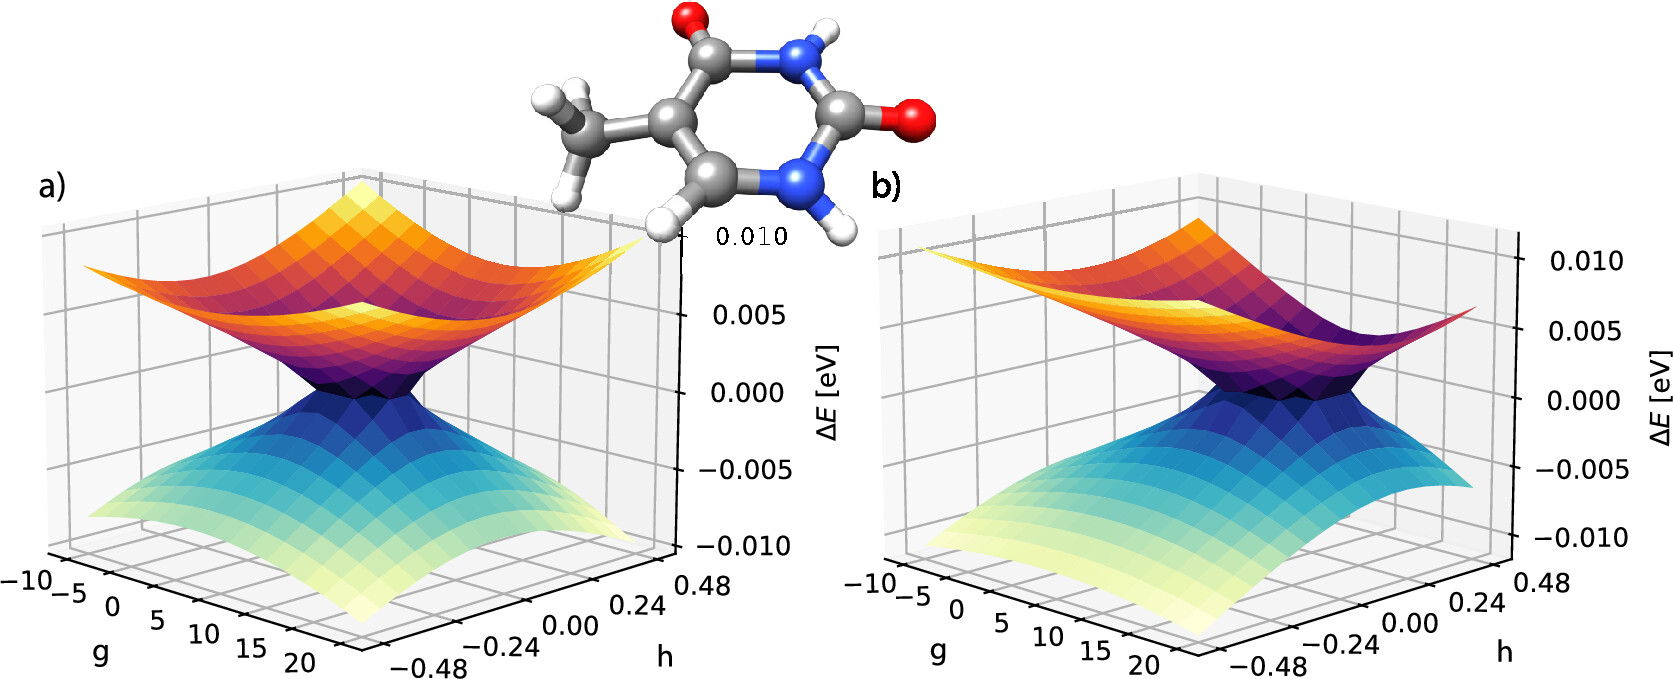
\includegraphics[width=0.8\textwidth]{images/CCSD.jpeg}
        \caption{Superficies de energía potencial S1 y S2 en timina calculadas con CCSD (a) y GCCSD (b).}
    \end{figure}
\end{frame}
